\section{臨界、原子炉と核データ}

\subsection{中性子増倍率}
\label{subsec:multipilication_factor}
核分裂連鎖反応では、核分裂の反応数が指数関数的に増減する。
1つの中性子が核分裂を引き起こし、2つの中性子が放出される体系を考える。この2つの核分裂中性子がどちらも
次の核分裂を起こす場合、この体系の中性子増倍率$k$は次のようになる。
\begin{equation}
  k = \frac{\text{発生した核分裂中性子のうち核分裂を起こす数}}{\text{核分裂を起こした中性子数}} = \frac{2}{1} = 2
\end{equation}
実際には核分裂反応はバラバラなタイミングで起こるが、簡単のために「世代」という概念を導入して考える。
丁度アニメーションのフレームと同じで、バラバラなタイミングで起こる核分裂反応を、あるタイミングで一気に
発生するものとして考える。1フレームあたりの時間は、核分裂が発生してから次の核分裂が発生するまでの平均的な
時間を使う。この時間を\emph{即発中性子寿命}、または\emph{世代時間}と呼ぶ。
中性子増倍率はある世代の中性子数を一つ前の世代の中性子数で割ったものとしても定義される。
\begin{equation}
  \label{eq:multi_factor}
  k = \frac{\text{ある世代の中性子数}}{\text{一つ前の世代の中性子数}}
\end{equation}
この中性子増倍率$k$が1より大きい状態を\emph{超臨界}、1より小さい状態を\emph{未臨界}、1の状態を\emph{臨界}と呼ぶ。
\[
k \; \left\{
  \begin{array}{ll}
    > 1 & \text{超臨界} \\
    = 1 & \text{臨界} \\
    < 1 & \text{未臨界}
  \end{array}
\right.
\]

\subsection{中性子と原子核の反応}
中性子は電荷を持たないため原子核に近づきやすく、原子核と\SI{e-12}{\centi\metre}程度まで近づくと
原子核と相互作用する。この相互作用は、大きく散乱反応(scattering)と吸収反応(absorption)に分けられる。

\subsubsection{散乱反応}
散乱反応はさらに\emph{弾性散乱}(elastic scattering)と\emph{非弾性散乱}(inelastic scattering)の2つに分けられる。
弾性散乱では中性子と原子核の運動エネルギーは保存されるため、一般には中性子の運動エネルギーの一部が原子核(ターゲット核)
に移り中性子の運動方向とエネルギーが変化する。弾性散乱には、中性子が原子核に取り込まれずに原子核のポテンシャルで散乱される
ポテンシャル散乱と、中性子が一旦原子核に取り込まれ複合核となった後にエネルギーを失わずに放出される共鳴散乱がある。
非弾性散乱ではターゲット核に移ったエネルギーの一部が原子核の励起エネルギーに使われる。
そのため、非弾性散乱は中性子のエネルギーがターゲット核の最低の励起エネルギーよりも大きい場合にのみ起こる。
Fig.~\ref{fig:neutron_scattering}は、いくつかの核種の弾性散乱断面積を示している。黒鉛のように配列的に並ぶ材料に
対しては、低エネルギー中性子は回析を起こす(干渉性散乱)。また、水分子の水素原子のように、結合によって
自由に動き回れないことによる断面積の変化も見られる(非干渉性非弾性散乱)。
中エネルギー領域の中性子に対しては核力のポテンシャルによって散乱し、断面積は一定の値を示す。
高エネルギーの領域の中性子に対しては核力のポテンシャルを超えて原子核に取り込まれる部分が出てくる。

Fig.~\ref{fig:neutron_inelastic_scattering}は、\ce{^{238}U}と\ce{^{90}Zr}の非弾性散乱断面積、
Fig.~\ref{fig:neutron_inelastic_scattering_U238}は\ce{^{238}U}の励起準位を考慮した非弾性散乱断面積を示している。


\begin{figure}[htbp]
  \centering
  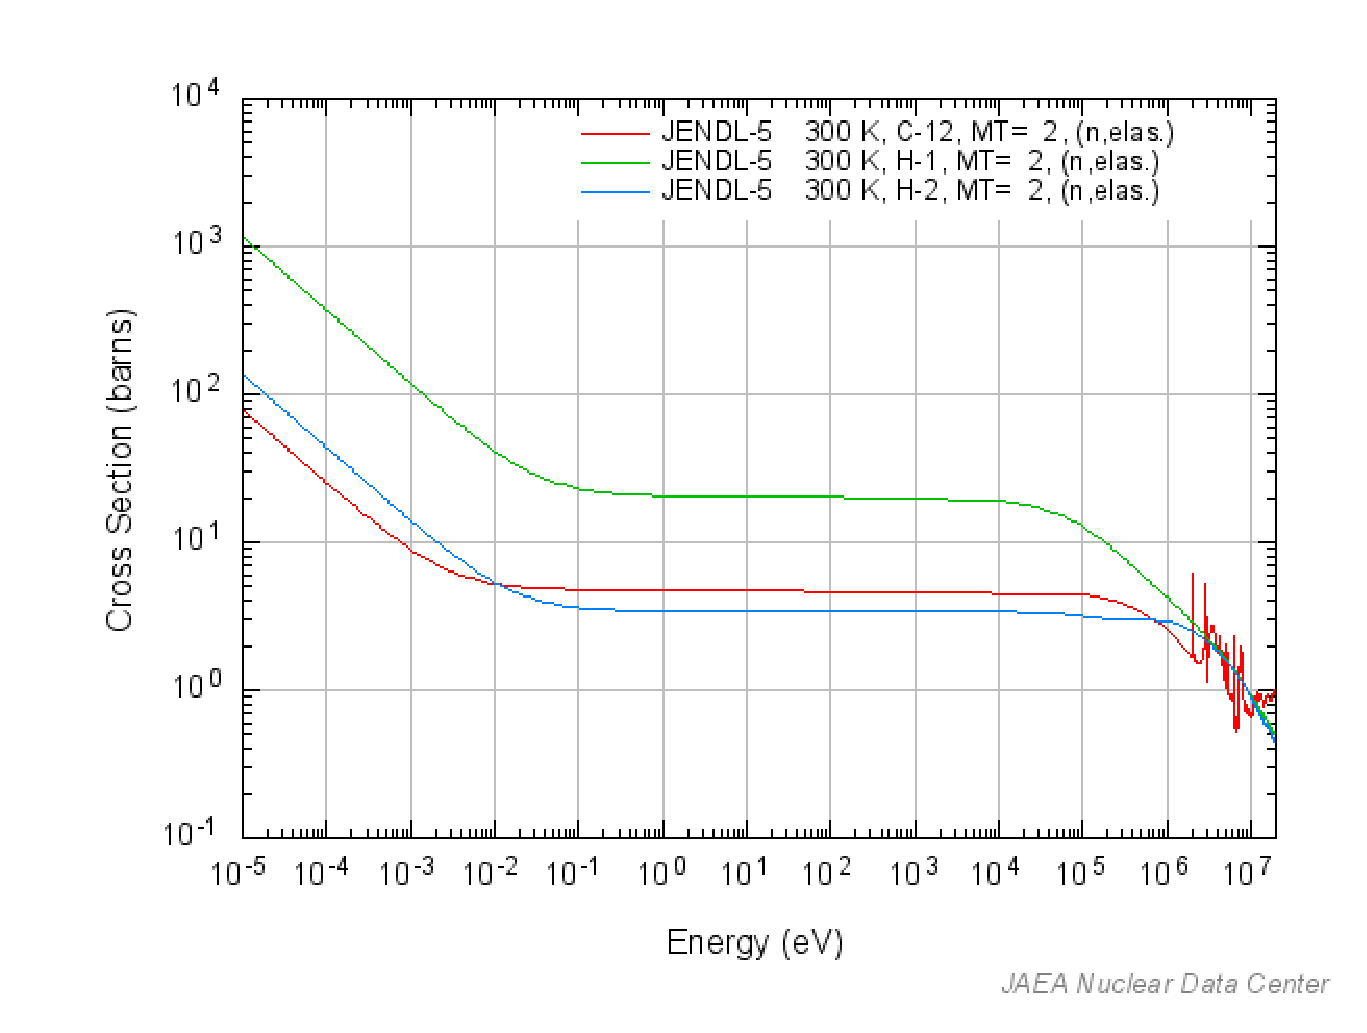
\includegraphics[width=0.8\textwidth]{figure/CrossSecElastic.eps}
  \caption{\ce{^{12}C},\ce{^{1}H},\ce{^{2}H}の弾性散乱(MT=2)の断面積}
  \label{fig:neutron_scattering}
\end{figure}

\begin{figure}[htbp]
  \centering
  \includegraphics[width=0.8\textwidth]{figure/U238Zr90Inela.eps}
  \caption{\ce{^{238}U},\ce{^{90}Zr}の非弾性散乱(MT=4)の断面積}
  \label{fig:neutron_inelastic_scattering}
\end{figure}

\begin{figure}[htbp]
  \centering
  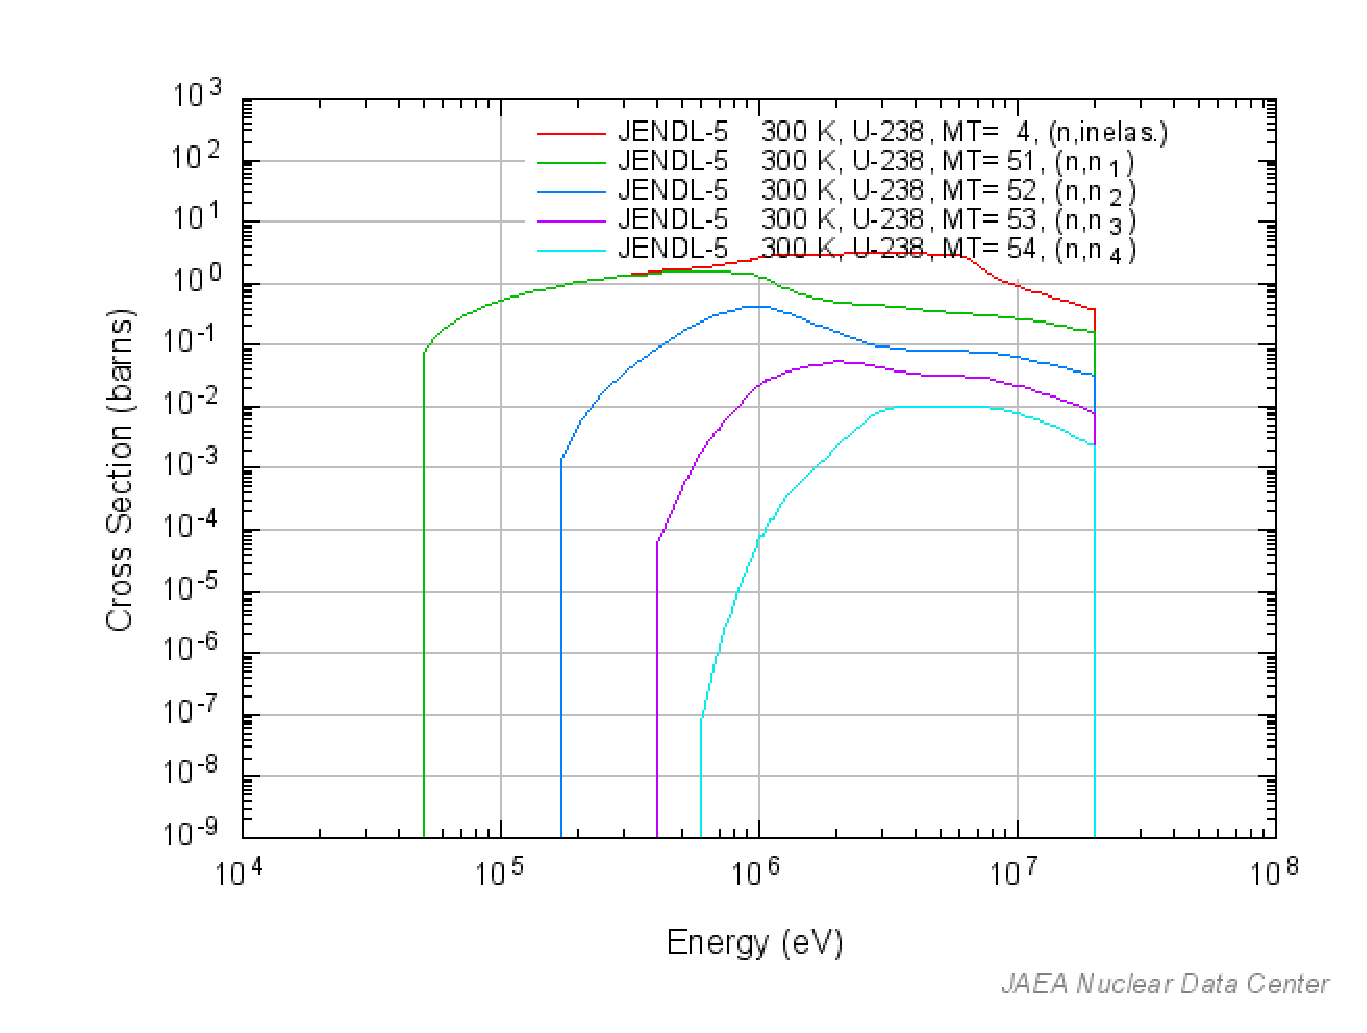
\includegraphics[width=0.8\textwidth]{figure/U238Inela_nx.eps}
  \caption{\ce{^{238}U}の非弾性散乱(MT=4,51,52,53,54)の断面積}
  \label{fig:neutron_inelastic_scattering_U238}
\end{figure}


\subsubsection{吸収反応}
原子核に中性子が取り込まれると、入射中性子のエネルギーと中性子の結合エネルギーの和の分だけ励起された複合核
が形成される。この複合核は不安定であるため、その後様々な反応を起こして安定な状態に戻ろうとする。
吸収反応この過程を経る反応の総称(散乱反応は除く)でその後の反応によってさらに多くの種類に分けられる。
これに分類されるものとしては、複合核から$\gamma$線を放出する放射捕獲反応、荷電粒子を放出する荷電粒子放出反応などがある。
原子炉において利用される核分裂反応や、入射中性子のエネルギーが高い場合に起こる2個以上の中性子が放出される反応も
この吸収反応に分類される。
Fig.~\ref{fig:neutron_absorption_Sm149}は、\ce{^{149}Sm}の(n,$\gamma$)反応、
Fig.~\ref{fig:neutron_capture_B10}は\ce{^{10}B}の(n,$\alpha$)反応、
Fig.~\ref{fig:neutron_fission}は\ce{^{235}U}の核分裂反応の断面積を示している。

それぞれの反応で共通して、低エネルギー領域では$1/v$に比例して断面積は減少している。
共鳴を持つ核種では中エネルギー領域で共鳴を起こすことも共通しているが、高エネルギー領域では捕獲断面積
は単調に減少するのに対し、核分裂断面積は階段状に増加することが分かる。
これは高エネルギーの中性子による核分裂反応では、中性子が吸収されてからすぐには割れず、1つ以上の中性子を
放出してから核分裂を起こす、マルチチャンス核分裂が存在するためである。
Fig.~\ref{fig:neutron_fission_U238}は、\ce{^{238}U}の核分裂反応において、分裂前に放出される
中性子の数ごとに分けた断面積(MT=19,20,21)と、すべての核分裂断面積の和(MT=18)を示している。

\begin{figure}[htbp]
  \centering
  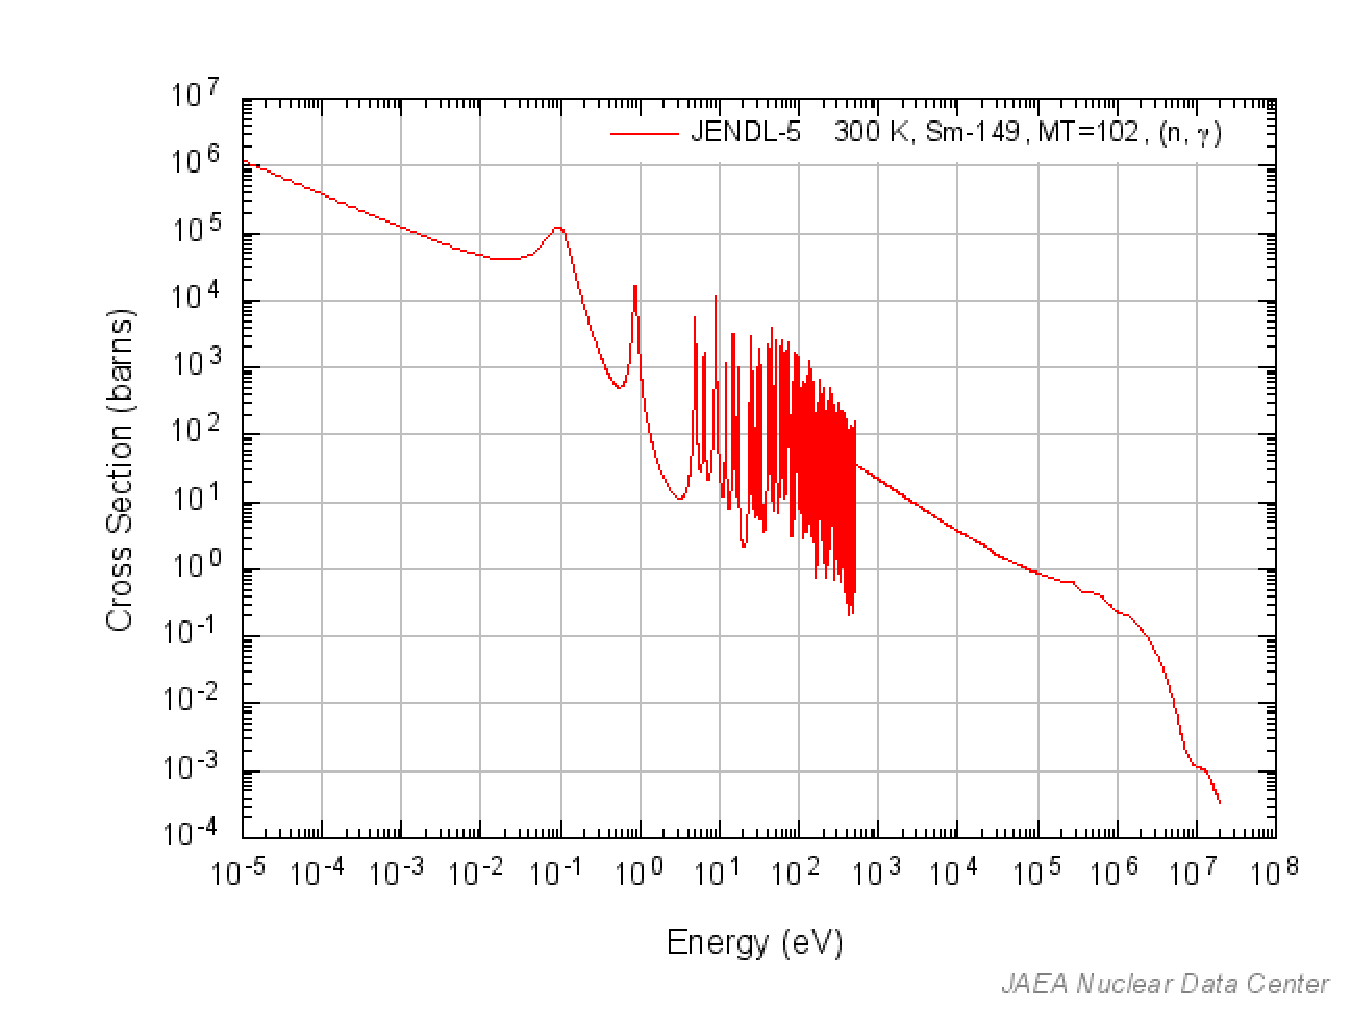
\includegraphics[width=0.8\textwidth]{figure/SmMT102.eps}
  \caption{\ce{^{149}Sm}の吸収反応(MT=102)の断面積}
  \label{fig:neutron_absorption_Sm149}
\end{figure}

\begin{figure}[htbp]
  \centering
  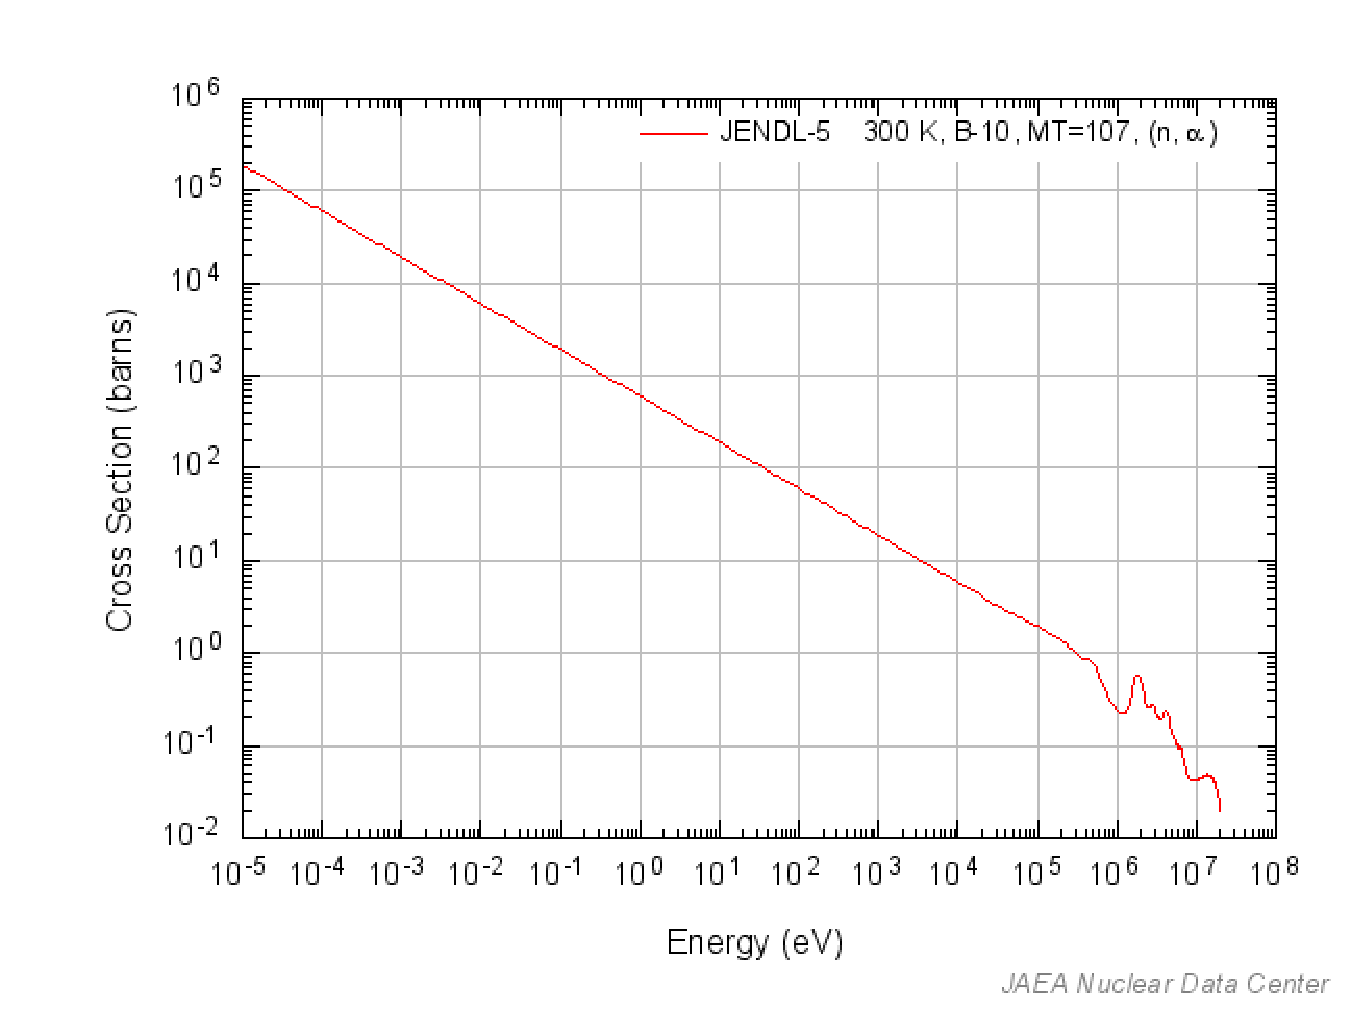
\includegraphics[width=0.8\textwidth]{figure/B10MT107.eps}
  \caption{\ce{^{10}B}の吸収反応(MT=107)の断面積}
  \label{fig:neutron_capture_B10}
\end{figure}

\begin{figure}[htbp]
  \centering
  \includegraphics[width=0.8\textwidth]{figure/U235Fission.eps}
  \caption{\ce{^{235}U}の核分裂反応(MT=18)の断面積}
  \label{fig:neutron_fission}
\end{figure}

\begin{figure}[htbp]
  \centering
  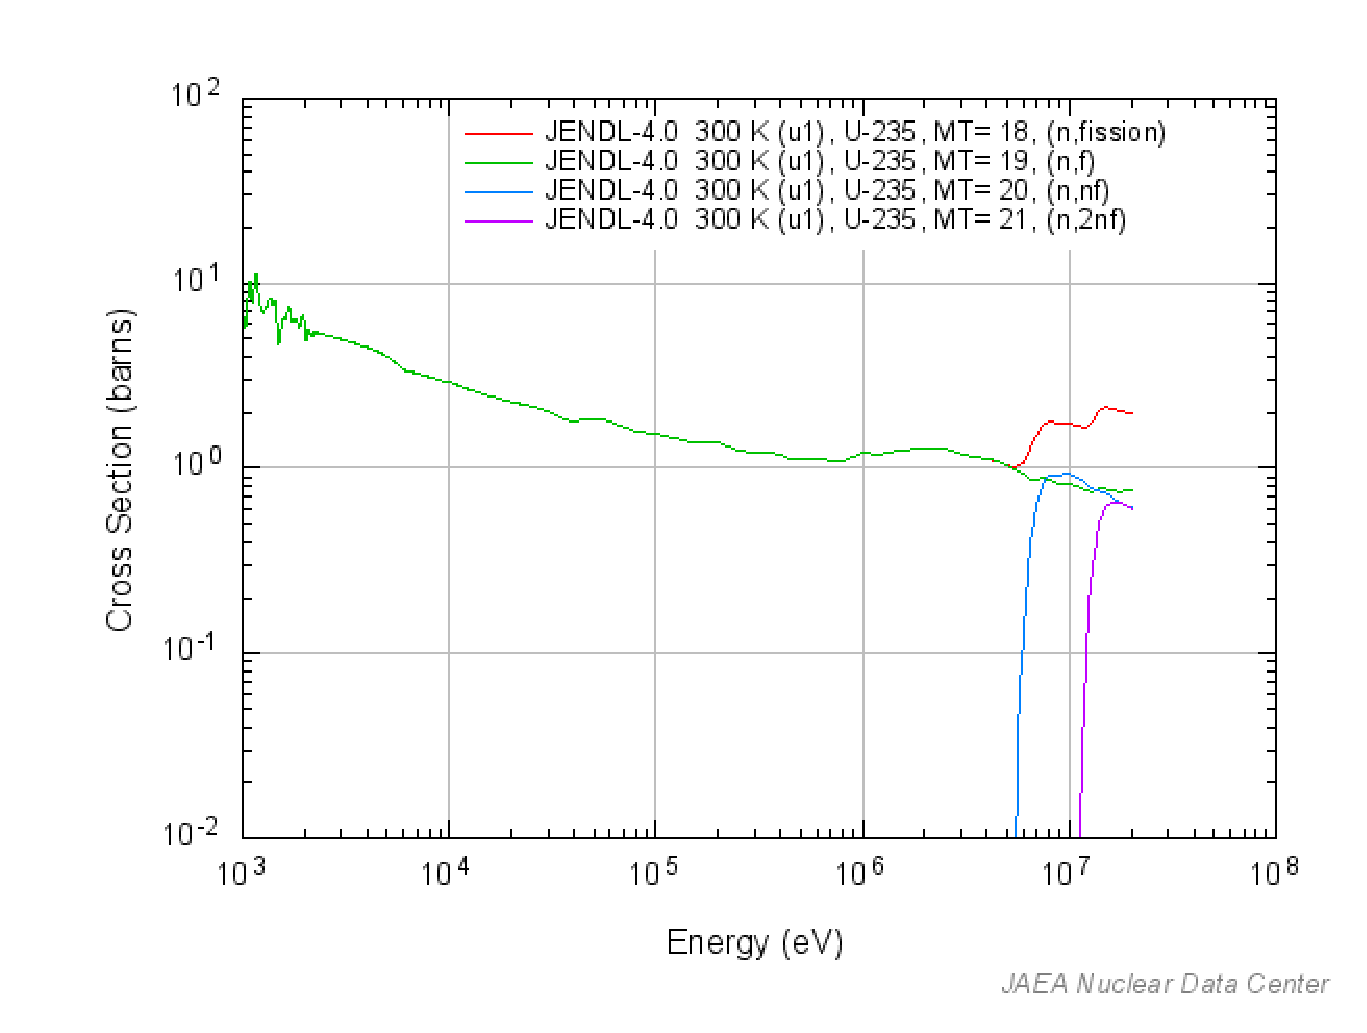
\includegraphics[width=0.8\textwidth]{figure/U235Fiss_xnf.eps}
  \caption{\ce{^{235}U}の核分裂反応(MT=18,19,20,21)の断面積}
  \label{fig:neutron_fission_U238}
\end{figure}

\subsection{臨界と中性子経済}
\ref{subsec:multipilication_factor}節で述べたように、臨界状態では中性子増倍率$k$は1で、
核分裂連鎖反応は外部から中性子を供給すること無しに、時間とともに増えも減りもせず一定の状態に維持される。
臨界を実現するための条件を調べるためにはFig.~\ref{fig:neutron_cycle}に示すような核分裂で発生した中性子の一生を考えることが適当である。

\begin{figure}[htbp]
  \centering
  \includegraphics[width=0.8\textwidth]{figure/neutron_cycle.eps}
  \caption{核分裂連鎖反応のサイクル}
  \label{fig:neutron_cycle}
\end{figure}

ある大きさの核分裂物質を含む体系を考える。
核分裂で発生したある世代の中性子は、体系から漏れるか、体系内にとどまるかのいずれかである。
体系にとどまる確率を$P_\text{NL}$とする。
体系にとどまった中性子は燃料に吸収されるか、燃料以外の物質に吸収されるかのいずれかである。
吸収されるとした場合に燃料に吸収される確率を$P_\text{aF}$とする。
燃料に吸収されたあと、それが捕獲反応ではなく核分裂反応を起こす確率を$P_\text{f}$とする。
核分裂を起こすと中性子を$\nu$個放出し、以下この過程を繰り返す。
\ref{equ:multi_factor}式より、増倍率$k$は次のように表される。
\begin{equation}
  k = P_\text{NL} \cdot P_\text{aF} \cdot P_\text{f} \cdot \nu
\end{equation}
以下この式をさらに定量的に考える。

\subsubsection{熱中性子利用率}
まず中性子が吸収される場合に、燃料に吸収される確率$P_\text{aF}$を考える。
燃料に吸収される確率は、燃料の中性子吸収断面積$\Sigma_\text{aF}$と、
体系全体の中性子吸収断面積$\Sigma_\text{a}$の比で表される。
\begin{equation}
  P_\text{aF} = \frac{\sigma_\text{aF}}{\sigma_\text{a}}
\end{equation}

% 章ごとの参考文献欄
\printbibliography[segment=\therefsegment,heading=subbibliography]

\newpage
